\begin{figure}[H]
	\centering
	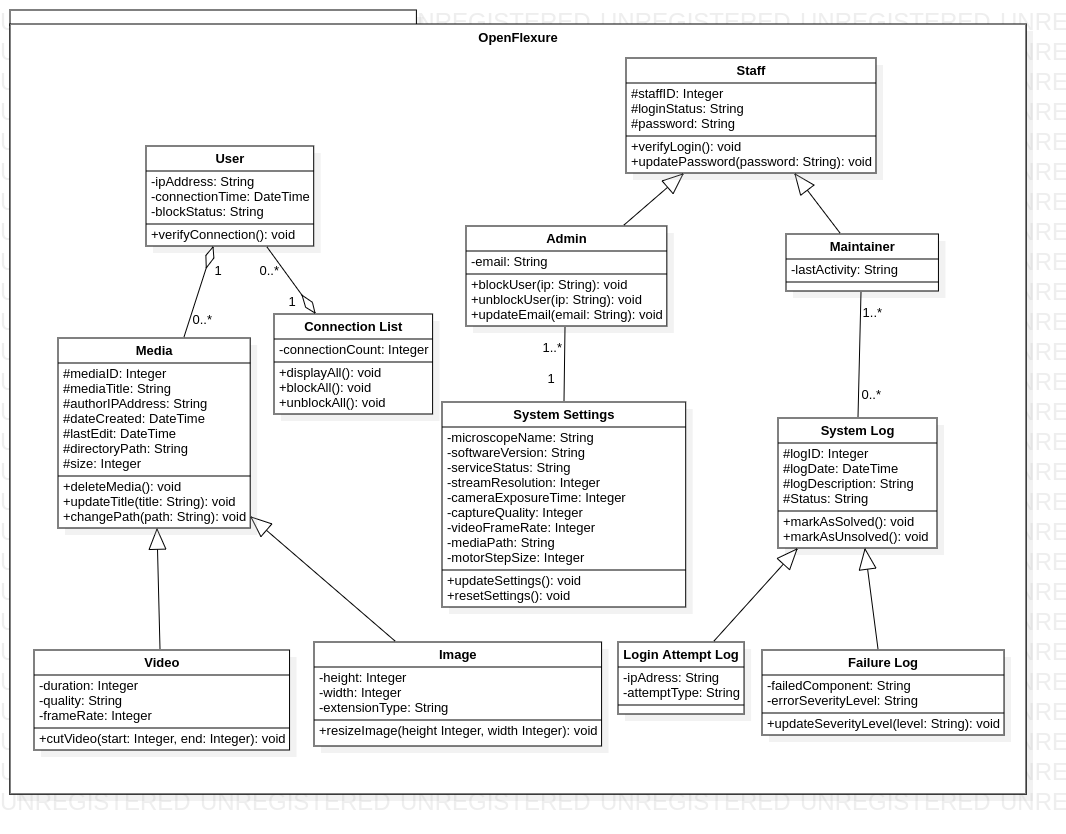
\includegraphics[scale=0.4]{Uml_Images/logical_db_class_diagram}
	\caption{Logical Database Requirements Class Diagram}
	\label{fig:logical_db_class_diagram}
\end{figure}

\begin{itemize}
	\item When a user connects to the microscope, a record that contains user's IP address, the time he/she connected to system and block status will be created in database. Initially, block status will be None. However, system admin can change the value of this attribute later by blocking/unblocking the user.
	\item Users cannot change any of these attributes.
	\item User records should be seen as connection records rather than profiles. Users do not require passwords or personal informations to connect the microscope. They are identified by their ip addresses.
	\item Connection list contains the list of users and number of connections.
	\item When user record is created, it is automatically added to the connection list.
	\item Connection list can be empty if there is no connection. It is not destroyed if there is no connection.
	\item If user disconnects, his/her record is automatically deleted from the database and connection list.
	\item When a user saves media, media records that contains metadata of the media will be created in the database. And authorIPAddress attribute of the media record will be initialized as the IP address of the user who saved the media.
	\item User may not have any media record associated with him/her. His/her record is not destroyed if there is no media record associated with him/her.
	\item When user record is deleted, the record of the media he/she saved is not destroyed. Furthermore, authorIPAddress attribute continues to keep IP address without pointing to user record.
	\item When user record is deleted, the record of the media he/she saved is not destroyed. Furthermore, authorIPAddress attribute continues to keep IP address without pointing to user record.
	\item Media class is generalization for Video and Image classes.
	\item mediaID is automatically created by the system and it is unique.
	\item User can only view the media created by him/her. Hence, he/she can only edit/delete the media associated with him/her.
	\item User cannot change the directory path. However, admins can change the path from the system settings.
	\item User can resize the image files by giving height and width parameter and cut the video files by giving starting time and ending time parameters. Again these files have to be associated by the user.
	\item Staff class is generalization for Admin and Maintainer classes.
	\item Each staff has unique staffID and passwords for signing in the system. Additionally, staff records contain loginStatus that indicates whether the staff is currently logged in or not.
	\item Staff can change their passwords. They cannot change their loginStatus and staffID.
	\item Admins have email addresses in addition to the attributes defined in Staff class. And they can change these email addresses.
	\item System settings record contains attributes for system wide settings. There is only one system settings record and it is created automatically when the system is established and cannot be deleted from the database.
	\item Only admins can update and reset system settings.
	\item Maintainer records have lastActivity field in addition to Staff attributes. It shows the last operation done by the maintainer. (e.g.,  viewed system log, checked updates etc.)
	\item System Log class is generalization for Login Attempt Log and Failure Log classes.
	\item System Log records contain unique logID, logDate, logDescription and status attributes. Status indicates whether the problem defined in the log is solved or not. Status field is initialized as unsolved.
	\item Maintainers can view system logs and update their status by marking them as solved or unsolved.
	\item Login Attempt Log contains IP address of the user attempted to login and attemptType that indicates whether user attempted to login as admin or maintainer.
	\item Failure Log contains failedComponent and errorSeverityLevel fields. errorSeverityLevel indicates the importance of the problem and it can be updated by the maintainers.

	
	

\end{itemize}